\section{CNN}
\subsection{卷积}
信号处理中,卷积被定义为:一个函数经过翻转和移动后与另一个函数的乘积的积分.
\begin{equation}
	(f*g)(t)=\int_{-\infty}^{\infty} f(\tau)g(t-tau)\mathrm{d}\tau 
\end{equation}
在深度学习中的卷积本质上是信号处理中的互相关(cross-correlation)操作。执行卷积的目的是从输入中提取有用的特征。卷积神经网络通过卷积在训练期间使用自动学习权重的函数来提取特征,所有这些提取出来的特征之后会被组合在一起做出决策。

\begin{enumerate}
	\item 2D卷积,如图\ref{2d_conv}
	\begin{figure}[H]
		\centering
		\label{2d_conv}
		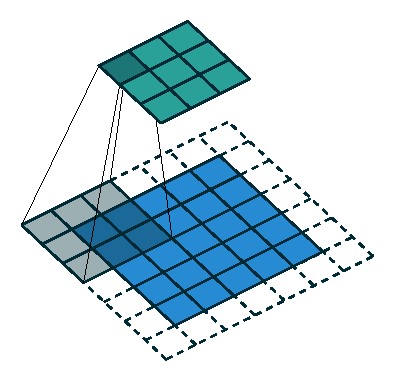
\includegraphics[width=0.3\linewidth]{./img/code/CNN/1.pdf}
		\caption{2D卷积}
	\end{figure}
	\item 多通道卷积(空间卷积),如图\ref{space_conv}
	\begin{figure}[H]
		\label{space_conv}
		\subfigure{
			\begin{minipage}[t]{\linewidth}
				\centering
				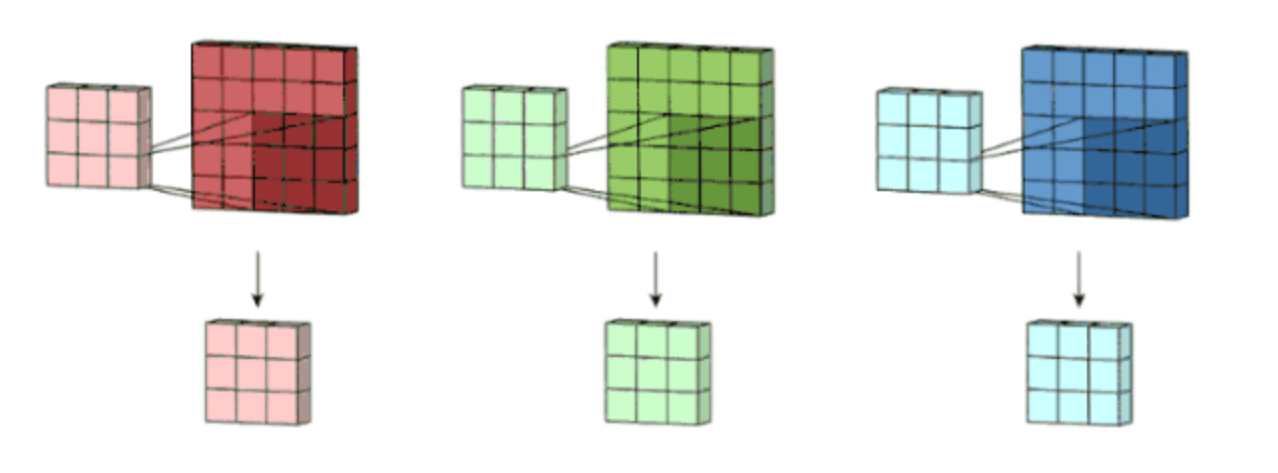
\includegraphics[width=0.5\linewidth]{./img/code/CNN/2-0}
			\end{minipage}	
		}
		
		\subfigure{
			\begin{minipage}[t]{\linewidth}
				\centering
				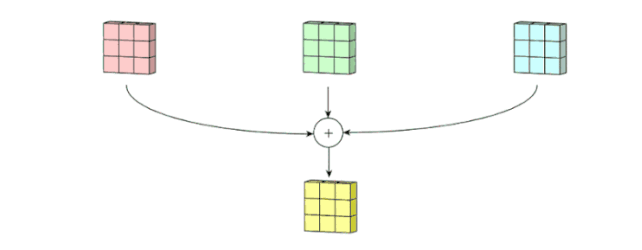
\includegraphics[width=0.5\linewidth]{./img/code/CNN/2-1}
			\end{minipage}	
		}	
		\caption{多通道卷积}
	\end{figure}
	\item 3D卷积,上面两种虽然实现了空间卷积,但是本质上还是2D卷积。而在3D卷积中,过滤器的深度要比输入层的深度要小,结果是,3D过滤器可以沿着3个方向移动。输出的数值同样也以3D空间的形式呈现,最终输出一个3D数据。如图\ref{3d_conv}.
	\begin{figure}[H]
		\centering
		\label{3d_conv}
		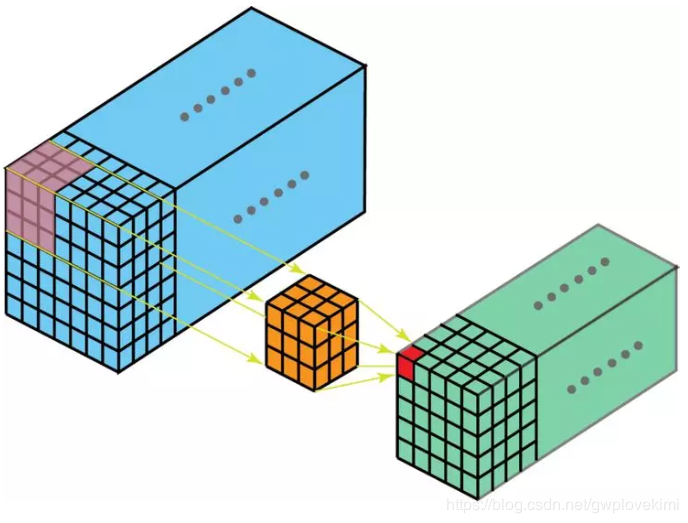
\includegraphics[width=0.3\linewidth]{./img/code/CNN/5}
		\caption{3D卷积}
	\end{figure}
	\item $1\times 1$卷积,计算上等于各个通道的加权和,同时可以改变特征通道数。如图\ref{1_conv}
	\begin{figure}[H]
		\label{1_conv}
		\centering
		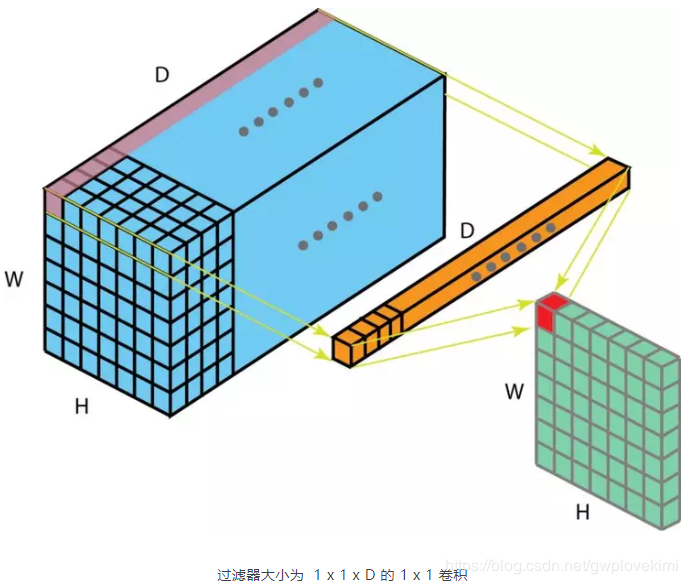
\includegraphics[width=0.3\linewidth]{./img/code/CNN/6}
		\caption{$1\times 1$卷积}
	\end{figure}
	\item 空间可分离卷积(Depthwise Separable Convolutions),我们可以将可分离卷积操作拆成多个步骤。减少计算量。如图\ref{space_sep_conv}
	\begin{figure}[H]
		\label{space_sep_conv}
		\centering
		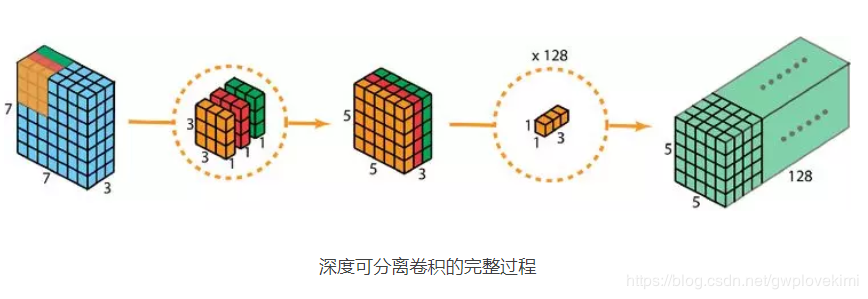
\includegraphics[width=0.5\linewidth]{./img/code/CNN/8}
		\caption{空间可分离卷积}
	\end{figure}
	\item 分组卷积(Group Convolutions),过滤器被拆分为不同中的组,每一个组负责具有一定深度的传统2D卷积的工作。另外,分组卷积也许有提供比标准完整2D卷积更好的模型。原因和稀疏过滤器有关。如图\ref{g_conv}
	\begin{figure}[H]
		\label{g_conv}
		\centering
		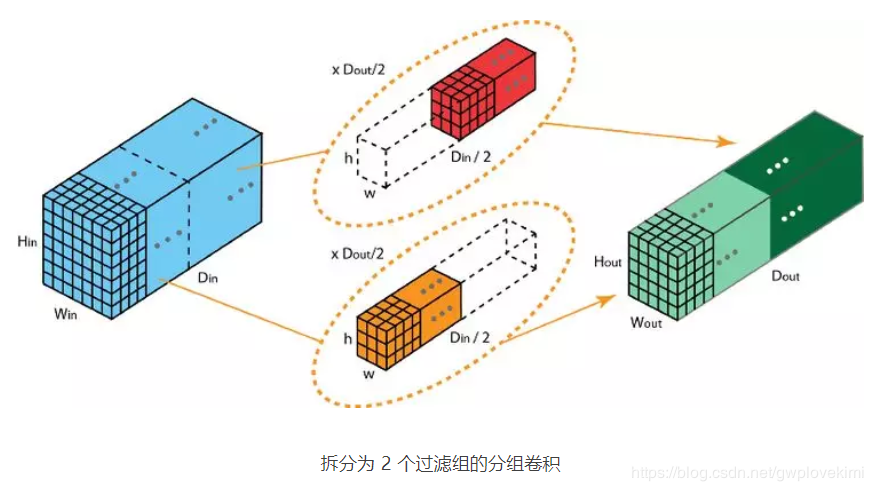
\includegraphics[width=0.5\linewidth]{./img/code/CNN/9}
		\caption{分组卷积}
	\end{figure}
	\item 扩张卷积(空洞卷积 Dilated Convolutions) ,引入另一个卷积层的参数被称为扩张率。这定义了内核中值之间的间距。扩张率为$2$的$3\times 3$的内核具有与$5\times 5$的内核相同的视野,而只使用9个参数。系统能以相同的计算成本,提供更大的感受野。如图\ref{d_conv}
	\begin{figure}[H]
		\label{d_conv}
		\centering
		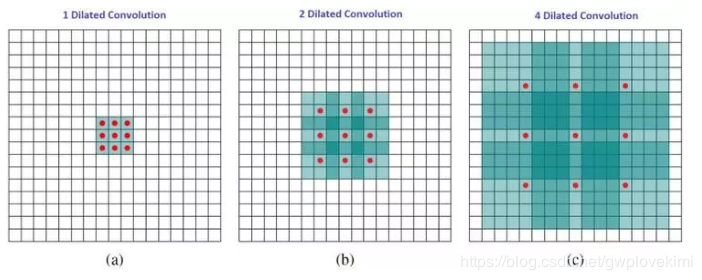
\includegraphics[width=0.5\linewidth]{./img/code/CNN/10}
		\caption{扩张卷积}
	\end{figure}
	\item 反卷积(转置卷积 Transposed Convolutions),转置卷积并非信号处理中的卷积运算的逆运算。对于 很多网络架构的很多应用言,我们往往需要进行与普通卷积方向相反的转换,即我们希望执行上采样。此时可以使用转置卷积操作。如图\ref{t_conv}
	\begin{figure}[H]
		\label{t_conv}
		\centering
		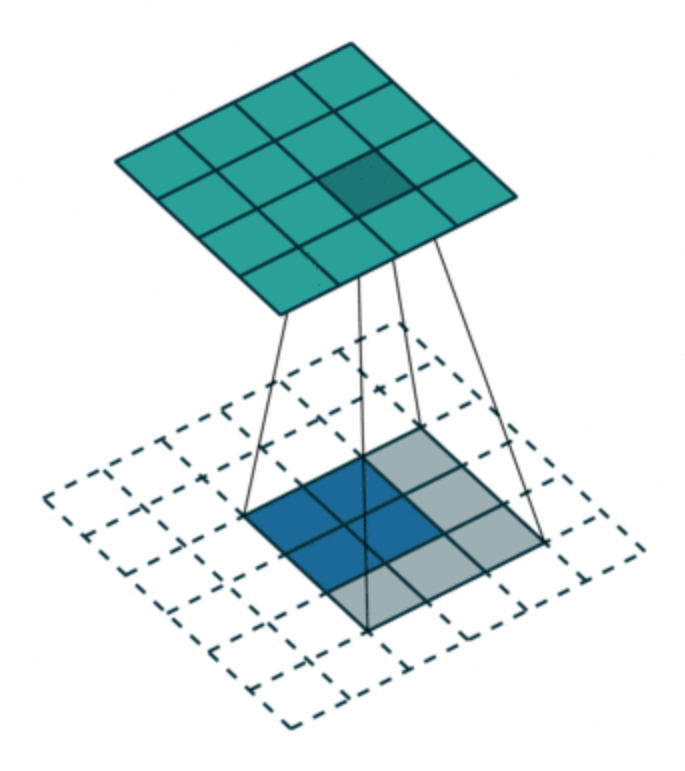
\includegraphics[width=0.3\linewidth]{./img/code/CNN/11.png}
		\caption{转置卷积}
	\end{figure}
\end{enumerate}
\subsection{卷积层的前向传播}
为简单起见,考虑单通道的情况
\begin{equation}
	\boldsymbol{X} * \boldsymbol{K} = \boldsymbol{Y}
\end{equation}
即
\begin{equation}
	\begin{pmatrix}
	x_{11}&  x_{12}& x_{13} \\ 
	x_{21}&  x_{22}&  x_{23}\\ 
	x_{31}&  x_{32}& x_{33}
	\end{pmatrix} * 
	\begin{pmatrix}
	k_{11}& k_{12} \\ 
	k_{21}& k_{22}
	\end{pmatrix} =
	\begin{pmatrix}
	y_{11}& y_{12} \\ 
	y_{21}& y_{22}
	\end{pmatrix} 
\end{equation}
这里
\begin{equation}
	\begin{aligned}
	\begin{pmatrix}
	y_{11}\\ 
	y_{12}\\ 
	y_{21}\\ 
	y_{22}
	\end{pmatrix} &= 
	\begin{pmatrix}
	x_{11}k_{11} +x_{12}k_{12} +x_{21}k_{21} +x_{22}k_{22} \\ 
	x_{12}k_{11} +x_{13}k_{12} +x_{22}k_{21} +x_{23}k_{22}\\
	x_{21}k_{11} +x_{22}k_{12} +x_{31}k_{21} +x_{32}k_{22}\\
	x_{22}k_{11} +x_{23}k_{12} +x_{32}k_{21} +x_{33}k_{22}
	\end{pmatrix}\\
	&=\begin{pmatrix}
	x_{11} &x_{12} &x_{21} &x_{22}  \\ 
	x_{12} &x_{13} &x_{22} &x_{23} \\
	x_{21} &x_{22} &x_{31} &x_{32} \\
	x_{22} &x_{23} &x_{32} &x_{33} 
	\end{pmatrix} \cdot 
	\begin{pmatrix}
	k_{11}\\ 
	k_{12}\\ 
	k_{21}\\ 
	k_{22}
	\end{pmatrix}
	\end{aligned}
\end{equation}
所以,卷积运算最终转化为矩阵运算。需要对原始的$\boldsymbol{X},\boldsymbol{K},\boldsymbol{Y}$进行变形操作,相应的记作$\boldsymbol{XC},\boldsymbol{KC},\boldsymbol{YC}$。多通道的情况只需要在维度上将操作扩展即可。
\subsection{卷积层的反向传播}
分析$\delta$误差反向传播过程可以简单的记忆为:如果神经网络$l+1$层某个结点的$\delta$误差要传到$l$层,我们就去找到前向传播时$l+1$层的这个结点和第$l$层的哪些结点有关系,权重是多少,那么反向传播时,$\delta$误差就会乘上相同的权重传播回来。

为了书写方便,记
\begin{equation}
	\begin{pmatrix}
		\delta_{11}\\ 
		\delta_{12}\\ 
		\delta_{21}\\ 
		\delta_{22}
	\end{pmatrix}=\nabla \boldsymbol{YC} = 
	\begin{pmatrix}
		\nabla y_{11}\\ 
		\nabla y_{12}\\ 
		\nabla y_{21}\\ 
		\nabla y_{22}
	\end{pmatrix}
\end{equation}
在反向传播中,$\delta$是从后面一层(一般是激活函数层或池化层)传过来的,是一个已知量,在此基础上求$\nabla \boldsymbol{K}, \nabla \boldsymbol{X}$
\begin{enumerate}
	\item 求$\nabla \boldsymbol{K}$
	\begin{equation}
		\nabla \boldsymbol{KC} = \boldsymbol{XC}^T\cdot \nabla \boldsymbol{YC}
	\end{equation}
	$\nabla \boldsymbol{KC}$ 只要reshape一下就可以得到$\nabla \boldsymbol{K}$
	\item 求$\nabla \boldsymbol{X}$
	
	根据反向传播公式,
	\begin{equation}
		\nabla \boldsymbol{XC} = \nabla \boldsymbol{YC} \cdot \boldsymbol{KC}^T
	\end{equation}
	但是,从$\nabla \boldsymbol{XC}$还原到$\nabla \boldsymbol{X}$不是一件容易的事,所以考虑新的计算方式。
	
	根据前向传播
	\begin{equation}
		\begin{pmatrix}
		y_{11}\\ 
		y_{12}\\ 
		y_{21}\\ 
		y_{22}
		\end{pmatrix} = 
		\begin{pmatrix}
		x_{11}k_{11} +x_{12}k_{12} +x_{21}k_{21} +x_{22}k_{22} \\ 
		x_{12}k_{11} +x_{13}k_{12} +x_{22}k_{21} +x_{23}k_{22}\\
		x_{21}k_{11} +x_{22}k_{12} +x_{31}k_{21} +x_{32}k_{22}\\
		x_{22}k_{11} +x_{23}k_{12} +x_{32}k_{21} +x_{33}k_{22}
		\end{pmatrix}
	\end{equation}
	可以计算每个$x_{ij}$的导数
	\begin{equation}
		\begin{aligned}
		\begin{pmatrix}
		\nabla x_{11} \\ 
		\nabla x_{12}\\ 
		\nabla x_{13}\\ 
		\nabla x_{21}\\ 
		\nabla x_{22}\\ 
		\nabla x_{23}\\ 
		\nabla x_{31}\\ 
		\nabla x_{32}\\ 
		\nabla x_{33}
		\end{pmatrix} &= \begin{pmatrix}
			k_{22}0 + k_{21}0 + K_{12}0+k_{11}\delta_{11} \\
			k_{22}0 + k_{21}0 + K_{12}\delta_{11}+k_{11}\delta_{12} \\
			k_{22}0 + k_{21}0 + K_{12}\delta_{12}+k_{11}0 \\
			k_{22}0 + k_{21}\delta_{11} + K_{12}0+k_{11}\delta_{21} \\
			k_{22}\delta_{11} + k_{21}\delta_{12} + K_{12}\delta_{21}+k_{11}\delta_{22} \\
			k_{22}\delta_{12} + k_{21}0 + K_{12}\delta_{22}+k_{11}0 \\
			k_{22}0 + k_{21}0 + K_{12}\delta_{21}+k_{11}0 \\
			k_{22}\delta_{21} + k_{21}\delta_{22} + K_{12}0+k_{11}0 \\
			k_{22}\delta_{22} + k_{21}0 + K_{12}0+k_{11}0 
		\end{pmatrix}\\
		&= \begin{pmatrix}
		0 & 0 & 0 & \delta_{11} \\ 
		0 & 0 & \delta_{11} & \delta_{12} \\ 
		0 & 0 & \delta_{12} & 0 \\ 
		0 & \delta_{11} & 0 & \delta_{21} \\ 
		\delta_{11} & \delta_{12} & \delta_{21} & \delta_{22} \\ 
		\delta_{12} & 0 & \delta_{22} & 0 \\ 
		0 & \delta_{21} & 0 & 0 \\ 
		\delta_{21} & \delta_{22} & 0 & 0 \\ 
		\delta_{22} & 0 & 0 & 0
		\end{pmatrix} \cdot 
		\begin{pmatrix}
			k_{11}\\ 
			k_{12}\\ 
			k_{21}\\ 
			k_{22}
		\end{pmatrix}
		\end{aligned}
	\end{equation}
	设上面三个矩阵分别为$\nabla \boldsymbol{X}^{'},\nabla \boldsymbol{Y}^{'},\nabla \boldsymbol{K}^{'}$,即$\nabla \boldsymbol{X}^{'}=\nabla \boldsymbol{Y}^{'}\cdot \nabla \boldsymbol{K}^{'}$。从而可见
	\begin{equation}
		\nabla \boldsymbol{X} = 
		\begin{pmatrix}
		\nabla x_{11}&\nabla  x_{12}&\nabla x_{13} \\ 
		\nabla x_{21}&\nabla  x_{22}&\nabla  x_{23}\\ 
		\nabla x_{31}&\nabla  x_{32}&\nabla x_{33}
		\end{pmatrix} = \begin{pmatrix}
		0 & 0 & 0 & 0 \\ 
		0 & \delta_{11} & \delta_{12} & 0 \\ 
		0 & \delta_{21} & \delta_{22} & 0 \\ 
		0 & 0 & 0 & 0
		\end{pmatrix} *
		\begin{pmatrix}
		k_{22} & k_{21} \\ 
		k_{12} & k_{11}
		\end{pmatrix} 
	\end{equation}
	这是一个卷积运算。不同的是对$\nabla \boldsymbol{Y}$进行卷积,从后向前卷积,有的文章称为逆向卷积。
\end{enumerate}

\subsection{池化层及池化层的反向传播}